\chapter{Appendix}
\label{cha:Appendix}

\section{Journal}
\label{sec:Journal}
\begin{table}[H]
    \centering
    \label{tab:Project Journal}
\begin{tabular}{||c | c | c || c||} 
 \hline
 Date &  Location & Duration & Activity \\ [0.5ex] 
 \hline\hline
  01.09.2023 & TBZ & 1.5h & Selected and bought \acs{devboard} \\ 
 \hline
 08.09.2023 & TBZ & 2h & Tested \acs{devboard} with demos \\ 
 \hline
  08.09.2023 & TBZ & 0.5h & Noted first ideas for \acs{dmm} \\ 
 \hline
   15.09.2023 & TBZ & 1.5h & Written and signed Project Agreement [\ref{sec:Project Agreement}] \\ 
 \hline
    21.09.2023 & Home & 3h & Created documentation template \\ 
 \hline
    22.09.2023 & TBZ & 2h &  Started writing Journal [\ref{sec:Journal}]\\ 
 \hline
    24.09.2023 & Home & 1.5h &  Made GANTT chart [\ref{sec:GANTT Chart}]\\ 
 \hline
    27.09.2023 & Home & 2h & Written detailed planning and introduction \\ 
 \hline
\end{tabular}
    \caption{Project Journal}
\end{table}
\newpage

\section{Project Agreement}
\label{sec:Project Agreement}
\begin{figure}[H]
	\centering
    \framebox{
	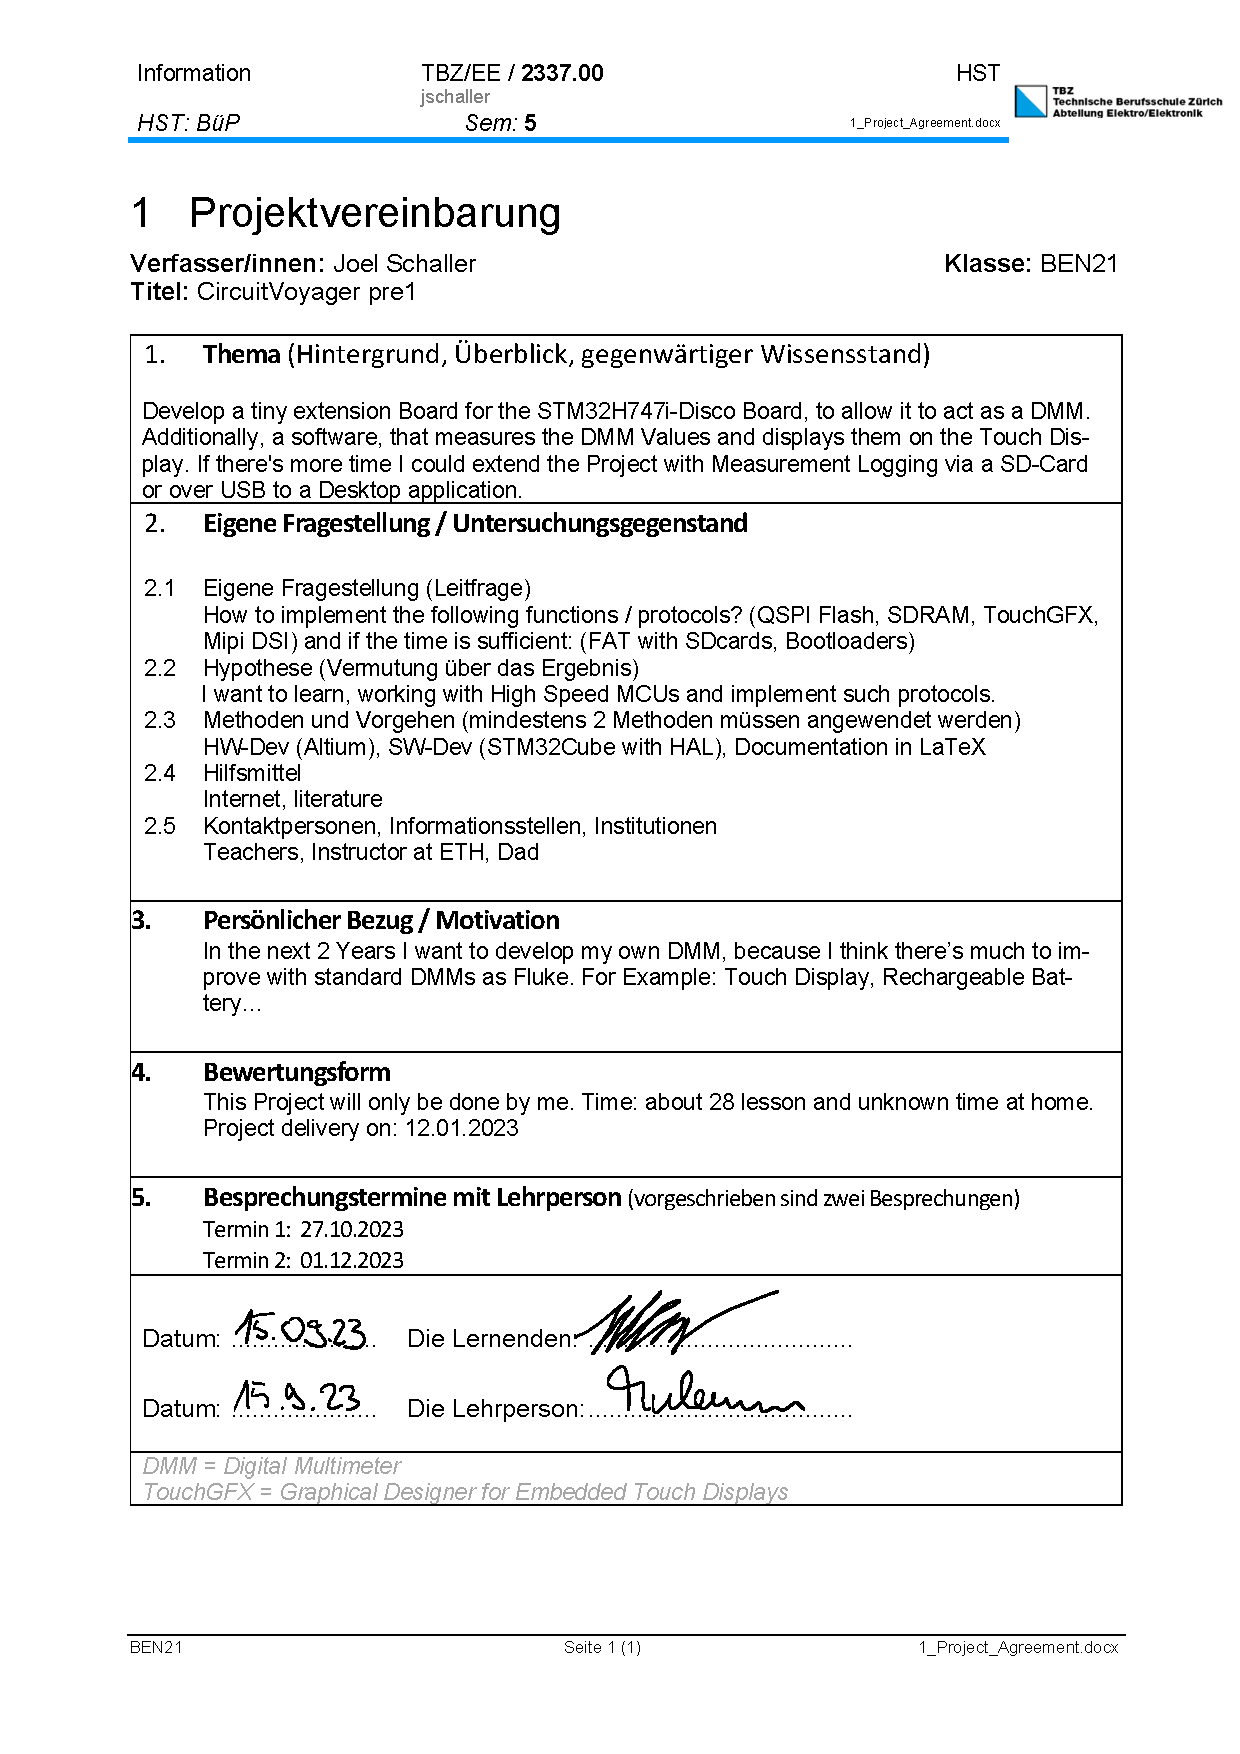
\includegraphics[width=14.5cm]{Resources/Other/1_Project_Agreement_CircuitVoyager_pre1_jschaller_230915.pdf}}
	\caption{Project Agreement}
	\label{fig:Project Agreement}
\end{figure}
\newpage

\section{GANTT Chart}
\label{sec:GANTT Chart}
\begin{figure}[H]
	\centering
    \framebox{
	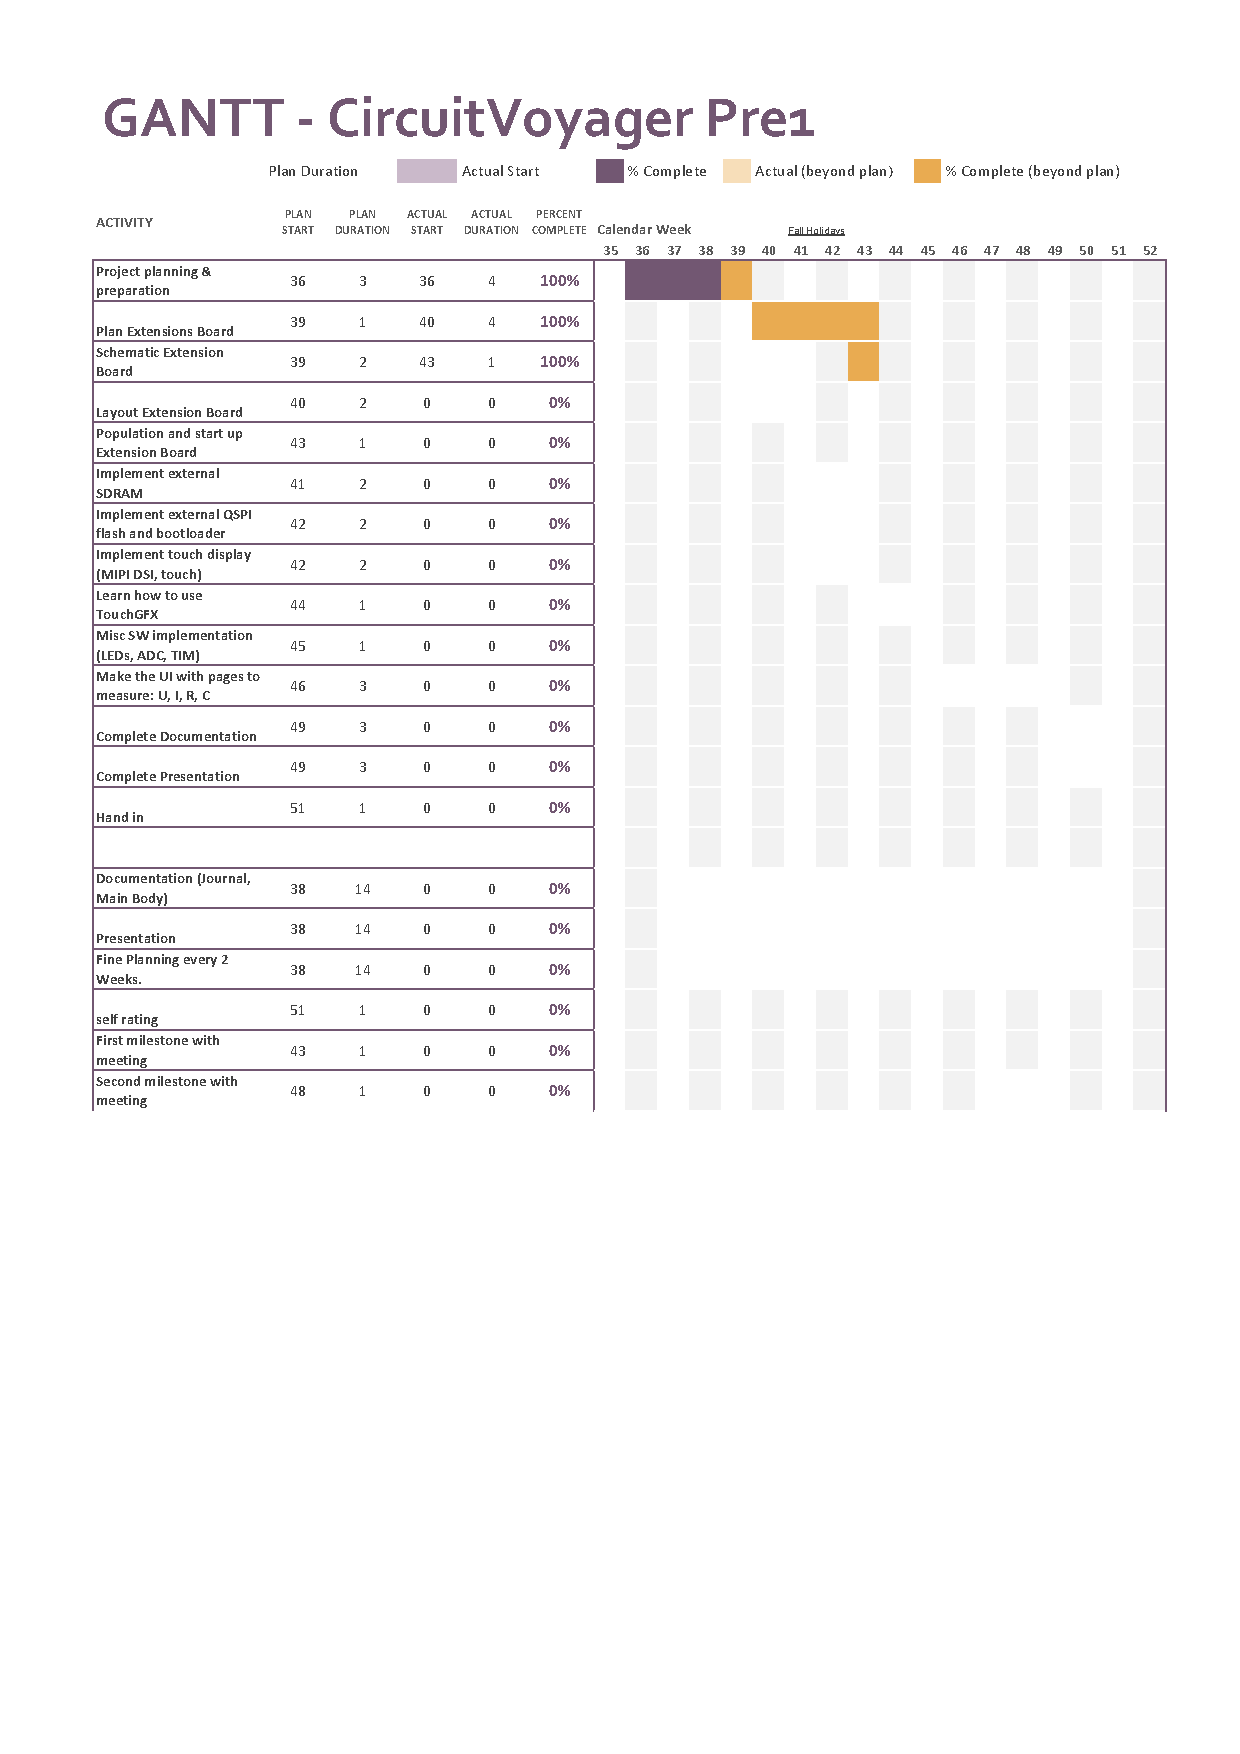
\includegraphics[width=14.5cm]{Resources/Other/GANTT.pdf}}
	\caption{GANTT Chart}
	\label{fig:GANTT Chart}
\end{figure}
\newpage

\section{Project Planning}
\label{sec:Project Planning}

\subsubsection{Cost}
I've already bought two \acs{devboard}s one of them stays at \acs{tbz} and the other is at home. One of these boards was paid by Mr. Malacarne. Further expenses from the \acs{pcb} will be paid by me and shouldn't exceed about 50 CHF, as the \acs{hw} isn't that complicated.

\subsubsection{Tools}
To realize this project I will mainly use, the \acs{sw} STM32CubeIDE with \acs{hal} and Altium Designer. The documentation is written in LaTeX in VSCode. And I'm planning to order the \acs{pcb} on JLCPCB and I will populate and reflow the PCB at ETHZ, where I'm also allowed to use the measurement equipment for the HW tests.

\subsubsection{When}
The most time of the project I will work at home because it's a rather big project to execute in one semester. I will also have much time in the fall holidays to work on it.


\subsection{KW39 \& 40}
\begin{itemize}
    \item Write introduction
    \item Planning: Cost, Tools, When, Why
    \item Create project diagram (learning process)
    \item ''Pflichtenheft''
    \item Documentation: Top bar as in EN-Poster
    \item Make a \acs{hw}-Digram for the Extension \acs{pcb}.
    \item Make the schematic of the Extension \acs{pcb}. 
    \begin{itemize}
        \item Part to measure voltage.
        \item Part to measure current.
        \item Part to measure resistance.
        \item Part to measure capacitance.
        \item Addressable LEDs.
    \end{itemize}
    \item Start with the Layout of the Extension \acs{pcb}.
\end{itemize}
\newpage